\documentclass[tikz,border=3pt]{standalone}
\usepackage[utf8]{inputenc}
\usepackage[T1]{fontenc}
\usepackage{libertinus}
\usepackage{amsmath,amssymb}
\usetikzlibrary{arrows.meta,calc,patterns,decorations.pathmorphing,decorations.markings,decorations.pathreplacing,bending}
\definecolor{UGblue}{RGB}{0,51,102}
\newcommand{\dbar}{\mathchar'26\mkern-12mu d}
\tikzset{
  >=Stealth,
  every node/.style={font=\small},
  caja/.style={draw,line width=0.9pt},
  pared/.style={draw,line width=1.6pt},
  ejes/.style={->,line width=0.8pt},
  adia/.style={draw,pattern=north east lines,pattern color=black!70,line width=0.5pt},
  gas/.style={fill=UGblue!8},
  punto/.style={fill,circle,inner sep=1.3pt},
  onda/.style={decorate,decoration={snake,amplitude=1.1pt,segment length=5pt,post length=3pt,pre length=0pt}},
}
\begin{document}
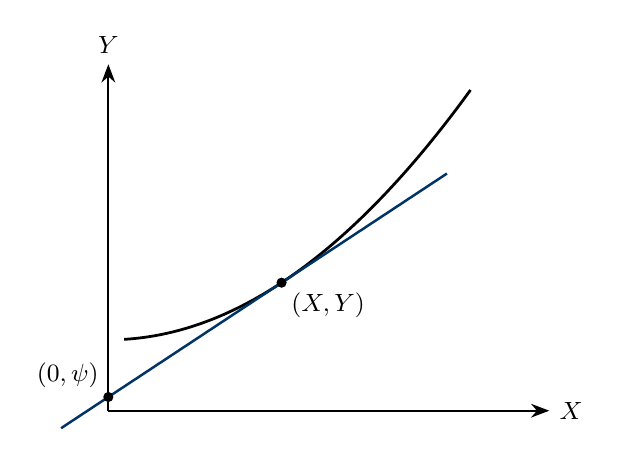
\begin{tikzpicture}
  \draw[ejes] (0,0) -- (5.6,0) node[right] {$X$};
  \draw[ejes] (0,0) -- (0,4.4) node[above] {$Y$};
  \draw[line width=1pt,domain=0.2:4.6,samples=50,smooth,variable=\x] plot ({\x},{0.15*\x*\x+0.9});
  \draw[line width=0.9pt,UGblue,domain=-0.6:4.3,variable=\t] plot ({\t},{1.6260+0.6600*(\t-2.20)});
  \node[punto] at (2.20,1.6260) {}; \node[punto] at (0,0.1740) {};
  \node[below right] at (2.20,1.6260) {$(X,Y)$};
  \node[above left] at (0,0.1740) {$(0,\psi)$};
\end{tikzpicture}
\end{document}
